% !Mode:: "TeX:UTF-8" 

\BiSection{2.8}{Figures}

\fancyhead[R]{本题2.8由QC.Z完成}

解:

\scalebox{3}{(a)}

$V_{TH}=V_{TH0}+\gamma(\sqrt{|2\Phi_F+V_{SB}|}-\sqrt{|2\Phi_F|})$

$I_1=I_D=\frac{1}{2}\mu_nC_{ox}\frac{W}{L}(V_{GS}-V_{TH})^2=\frac{1}{2}\mu_nC_{ox}\frac{W}{L}[V_{GS}-V_{TH0}-\gamma(\sqrt{|2\Phi_F+V_{SB}|}-\sqrt{|2\Phi_F|})]^2=\frac{1}{2}\mu_nC_{ox}\frac{W}{L}[V_{GS}-V_{TH0}-\gamma(\sqrt{|2\Phi_F+V_{DD}-V_{out}-V_{in}|}-\sqrt{|2\Phi_F|})]^2$

		\begin{figure}[H] %H为当前位置,!htb为忽略美学标准,htbp为浮动图形
	\begin{minipage}{\linewidth}
		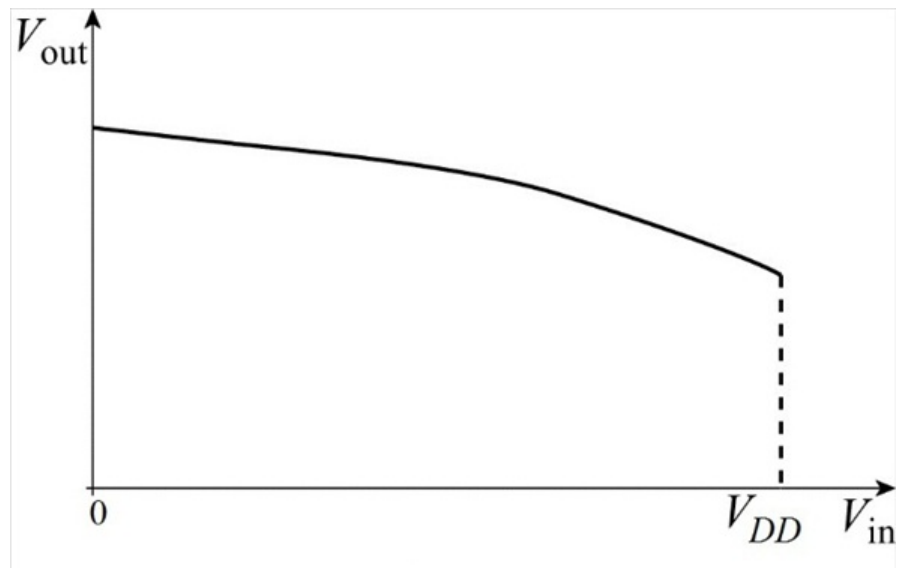
\includegraphics{2.8-1}
	\end{minipage}
	\caption*{图1} %最终文档中希望显示的图片标题
\end{figure}

\scalebox{3}{(b)}

$V_{out}=V_{DD}-R_1I_1=3-R_1I_1=3-R_1\{\frac{1}{2}\mu_nC_{ox}\frac{W}{L}[V_{GS}-V_{TH0}-\gamma(\sqrt{|2\Phi_F+V_{SB}|}-\sqrt{|2\Phi_F|})]^2\}=3-R_1\{\frac{1}{2}\mu_nC_{ox}\frac{W}{L}[1-0.7-0.45(\sqrt{|0.9+1-V_{in}|}-\sqrt{|0.9|})]^2\}=3-R_1\{\frac{1}{2}\mu_nC_{ox}\frac{W}{L}[0.3-0.45(\sqrt{1.9-V_{in}}-\sqrt{0.9})]^2\}$

		\begin{figure}[H] %H为当前位置,!htb为忽略美学标准,htbp为浮动图形
	\begin{minipage}{\linewidth}
		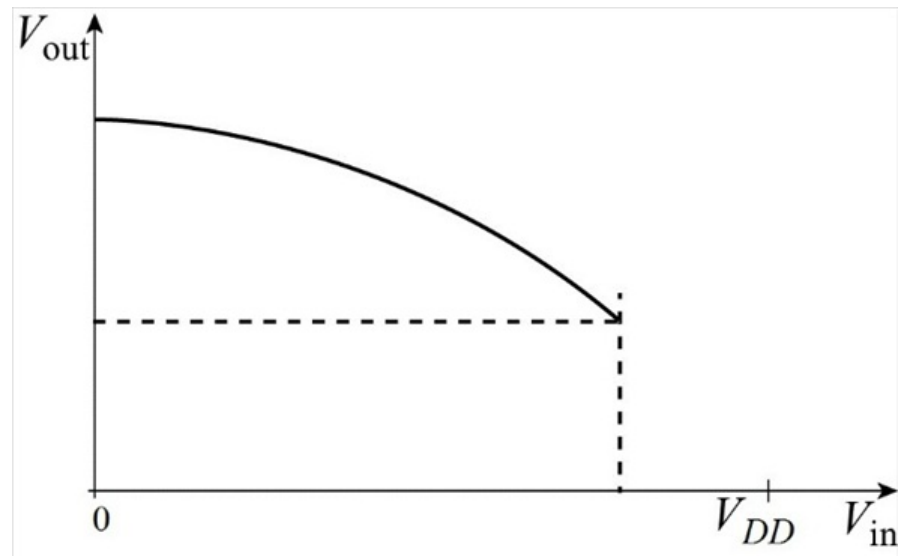
\includegraphics{2.8-2}
	\end{minipage}
	\caption*{图2} %最终文档中希望显示的图片标题
\end{figure}

\scalebox{3}{(c)}

NFET源漏交换

		\begin{figure}[H] %H为当前位置,!htb为忽略美学标准,htbp为浮动图形
	\begin{minipage}{\linewidth}
		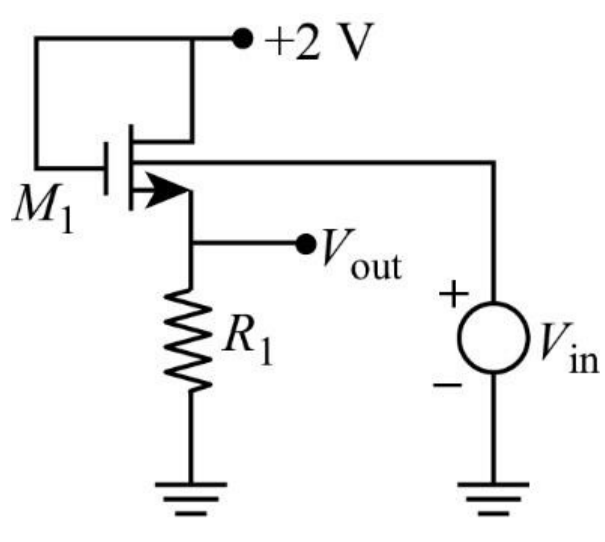
\includegraphics{2.8-3}
	\end{minipage}
	\caption*{图3} %最终文档中希望显示的图片标题
\end{figure}

$\frac{V_{out}}{R_1}=I_D=\frac{1}{2}\mu_nC_{ox}\frac{W}{L}(V_{GS}-V_{TH})^2=\frac{1}{2}\mu_nC_{ox}\frac{W}{L}\{2-V_{out}-[V_{TH0}+\gamma(\sqrt{|2\Phi_F+V_{SB}|}-\sqrt{|2\Phi_F|})]\}^2=\frac{1}{2}\mu_nC_{ox}\frac{W}{L}\{2-V_{out}-[0.7+0.45(\sqrt{|0.9+V_{out}-V_{in}|}-\sqrt{|0.9|})]\}^2$

		\begin{figure}[H] %H为当前位置,!htb为忽略美学标准,htbp为浮动图形
	\begin{minipage}{\linewidth}
		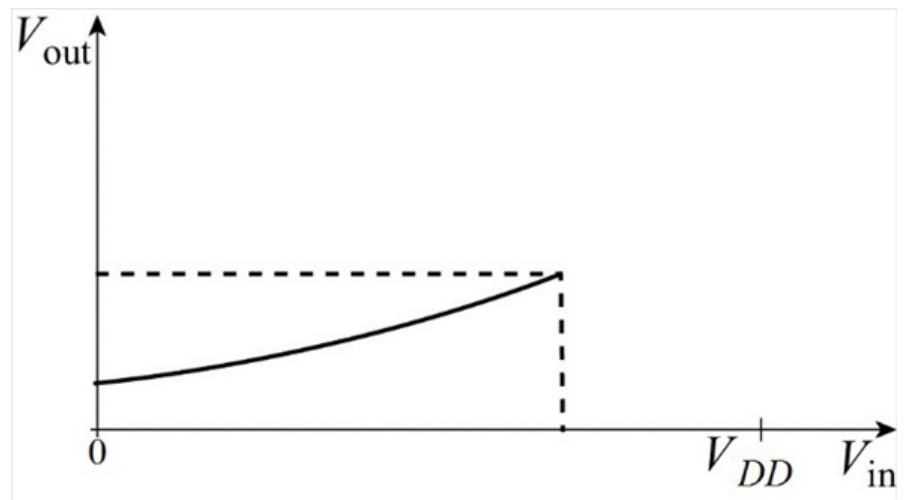
\includegraphics{2.8-4}
	\end{minipage}
	\caption*{图4} %最终文档中希望显示的图片标题
\end{figure}